\documentclass[11pt]{article}

% \usepackage[sort]{natbib}
\usepackage[style=verbose]{biblatex}
\usepackage{fancyhdr}
\usepackage{graphicx,caption,subcaption,color,float} %Graphics stuff
\usepackage{hyperref,amssymb,amsmath, amsfonts, amsthm, enumerate, bm}
\usepackage{placeins, cancel, wrapfig, xcolor, array, multirow, booktabs, algorithm, algpseudocode} 
\usepackage[margin=0.9in]{geometry}
\usepackage{ulem}
\graphicspath{ {figs/} }
\bibliography{references}

% you may include other packages here (next line)
\usepackage{enumitem}
\usepackage{dirtytalk}
\usepackage{amsmath}
%----- you must not change this -----------------
\topmargin -1.0cm
\textheight 23.0cm
\parindent=0pt
\parskip 1ex
\renewcommand{\baselinestretch}{1.1}
\pagestyle{fancy}
\renewcommand{\theenumi}{\Alph{enumi}}
\makeatletter
\newcommand{\distas}[1]{\mathbin{\overset{#1}{\kern\z@\sim}}}%
\newsavebox{\mybox}\newsavebox{\mysim}
\newcommand{\distras}[1]{%
	\savebox{\mybox}{\hbox{\kern3pt$\scriptstyle#1$\kern3pt}}%
	\savebox{\mysim}{\hbox{$\sim$}}%
	\mathbin{\overset{#1}{\kern\z@\resizebox{\wd\mybox}{\ht\mysim}{$\sim$}}}%
}
\makeatother
%----------------------------------------------------

% enter your details here----------------------------------
\lhead{}
\chead{}
\rhead{}
\lfoot{}
\cfoot{}
\rfoot{}
\setlength{\fboxrule}{4pt}\setlength{\fboxsep}{2ex}
\renewcommand{\headrulewidth}{0.4pt}
\renewcommand{\footrulewidth}{0.4pt}


\title{Homework 1}
\author{Priyesh Rajesh Kakka}

\begin{document}
	
	\maketitle
	
	\textbf{Problem 1:}
	
	Katz centrality us defined as \\
	
	\begin{equation}
		\label{eqn: 1}
		\boldsymbol{c}_{K a t z}=\beta(\boldsymbol{I}-\alpha \boldsymbol{A})^{-1} \overrightarrow{\mathbf{1}}
	\end{equation}
	
	and the expansion of the RHS in the above equation is defined as 
	
	\begin{equation}
		\boldsymbol{c} = (\mathbf{I}-\alpha A)^{-1} \mathbf{1}=\mathbf{1}+\alpha A \mathbf{1}+\alpha^2 A^2 \mathbf{1}+\ldots
	\end{equation}
	where $\beta$ is constant. 
	The divergence of the series would happen when $\operatorname{det}(\mathbf{I}-\alpha A)=0$, whose roots are $\alpha^{-1}$ which are eigen value of A.\\
	The limit at which series would diverge is when $\alpha = 1/\kappa$ where $\kappa$ is the largest principle eigen value of A. Hence equation~\ref{eqn: 1} will converge for $\alpha \in\left[0, \kappa^{-1}\right)$ as for $\alpha$ when 0 would make katz centrality uniform throughout the graph based on constant $\beta$.
	
	
	\clearpage
	
	
	\textbf{Problem 2:}
	
	For finding common neighbours we can use the concept of walk with length 2. Hence, relation to compute total number of common neighbours $\left|N\left(v_i\right) \cap N\left(v_j\right)\right|$ between nodes $v_i$ and $v_j$ is given as 
	\begin{equation}
		\label{eqn: 2}
		\begin{aligned}
			N_{i j}^{(2)} &=\sum_{k=1}^n A_{i k} A_{k j} \\
			&=\left[A^2\right]_{i j}
		\end{aligned}...\text{From lec 1 slides}
	\end{equation}
	\clearpage
	
	\textbf{Problem 3:}
	
	Jaccard's local overlap similarity is given as 
	\begin{equation}
		S_{i j}^{\mathrm{Jaccard}}=\frac{\left|N\left(v_i\right) \cap N\left(v_j\right)\right|}{\left|N\left(v_i\right) \cup N\left(v_j\right)\right|}
	\end{equation}
	
	Where numerator $\left|N\left(v_i\right) \cap N\left(v_j\right)\right|$ is given by equation~\ref{eqn: 2} and the denominator $\left|N\left(v_i\right) \cup N\left(v_j\right)\right| = d_{i} + d_{j} - \left|N\left(v_i\right) \cap N\left(v_j\right)\right|$. Here $d_{i}$ is the degree of vertex $v_{i}$. 
	
	
	Coding for the same, one gets similarity matrix as,
	
	\begin{figure}[!h]
		\centering
		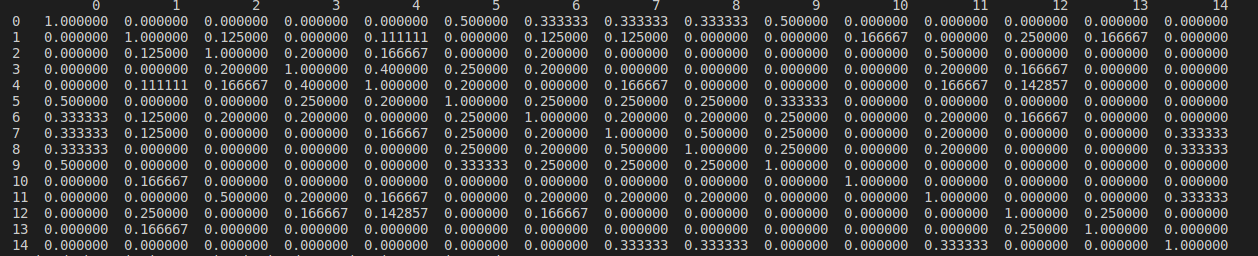
\includegraphics[scale=0.3]{Similarity_matrix.png}
		\caption{Similarity matrix}
		\label{fig:similarity matrix}
	\end{figure}

and the labels for similarity matrix~\ref{fig:similarity matrix} is given by figure~\ref{fig:my_label}. 

	\begin{figure}
	\centering
	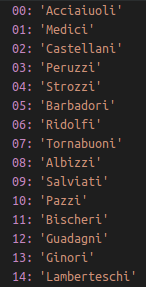
\includegraphics[scale=0.7]{labels.png}
	\caption{Label for similarity matrix}
	\label{fig:my_label}
\end{figure}

	and similarity between ”Ginori” family and other families in the Florentine Families graph is given by figure~\ref{Ginori_similar},
	
	\begin{figure}
	\centering
	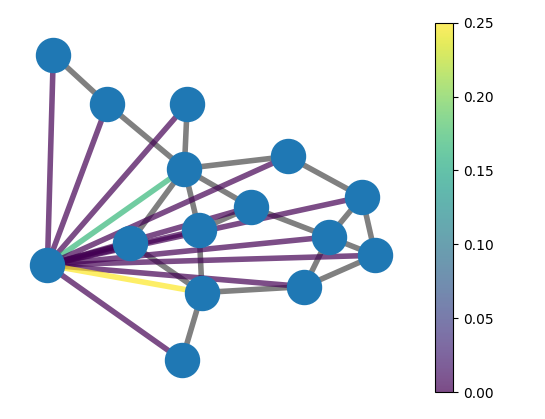
\includegraphics[scale=0.5]{Ginori.png}
	\caption{similarity between ”Ginori” family and other families}
	\label{Ginori_similar}
\end{figure}	
	
\end{document}